\documentclass[10pt]{article}
%	options include 12pt or 11pt or 10pt
%	classes include article, report, book, letter, thesis

\usepackage[a4paper,bindingoffset=0.2in,%
left=1in,right=1in,top=0.2in,bottom=0.3in,%
footskip=.15in]{geometry}

\usepackage[T1]{fontenc}
\usepackage[polish]{babel}
\usepackage[utf8]{inputenc}
\usepackage{lmodern}
\usepackage{pgfplots}
\usepackage{graphicx}
\usepackage{amsmath}
\usepackage{subcaption}
\usepackage{multirow}
\usepackage{hyperref}
\usepackage{mathtools}
\newtheorem{hip}{Hipoteza}
\newtheorem{que}{Pytanie}
\newtheorem{wn}{Wniosek}
\newtheorem{wyd}{Zadanie}
\title{Algorytmy numeryczne}
\author{Zadanie 3 \\ Dawid Bińkuś \& Oskar Bir \& Mateusz Małecki\\grupa 1 tester-programista}
\date{9 Grudzień 2018}

\begin{document}
\maketitle 

\section{Majority/Consensus problem}
Sprawozdanie prezentuje analizę problemu przeprowadzenia głosowania większościowego. W tym celu, stworzony został program, który generuje układ równań dla danego ustawienia oraz oblicza prawdopodobieństwo zagłosowania na TAK.

\section{Implementacja i możliwość stosowania metod iteracyjnych}
\begin{figure}[h]
	\caption{Wykres reprezentujący błąd bezwzględny metod Gaussa oraz metod iteracyjnych względem metody MonteCarlo\label{rys}}
	\begin{subfigure}{1\textwidth}
		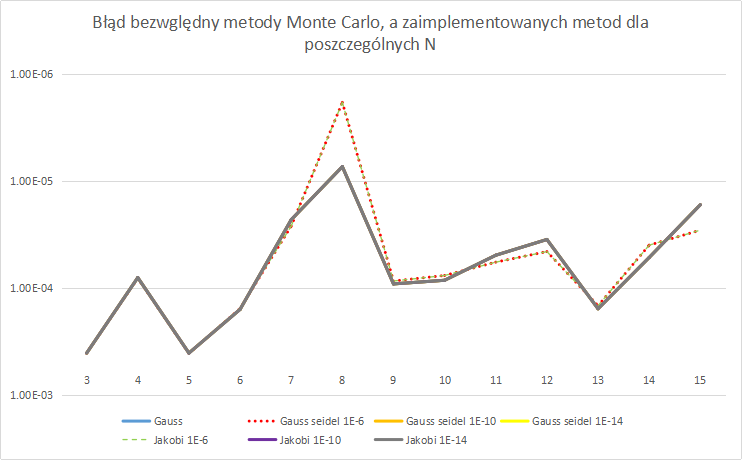
\includegraphics[width=\textwidth]{1.png}
		\caption{ \label{Rys1a}}
	\end{subfigure}
\end{figure}
\subsection{Generowanie układu równań dla danej liczby agentów}
Generowanie układu równań dla danego $N$ odbywa się w sposób następujący:
\begin{enumerate}
	\item Określenie wszystkich możliwych przypadków (ilość agentów $\#Y$ oraz ilość agentów $\#N$),
	\item Wyliczenie wszystkich możliwych kombinacji bez powtórzeń za pomocą Symbolu Newtona ${{N} \choose {2}}$,
	\item Wygenerowanie równań dla poszczególnych przypadków,
	\item Osadzenie równań w macierzy
	\item Wypełnienie wektora $B$ zerami z wyjątkiem ostatniej wartości (gdyż ostatni przypadek jest zawsze przypadkiem pewnym, tj $P_{\#Y=N,\#N=0}=1)$
\end{enumerate}
\subsection{Prawidłowość implementacji}
By zweryfikować poprawność implementacji zarówno generowania macierzy jak i obliczania stworzonego w ten sposób układu równań, wykonane zostały testy dla $N \in [3,15]$, których zadaniem było obliczenie wszystkich możliwych prawodopodobieństw i zestawienie ich z prawdopodobieństwem wyliczonym za pomocą metody MonteCarlo w ilości iteracji $=1000000$
Błędy osiągnięte za pomocą metod Gaussa \ref{Rys1a} osiągają wartości rzędu $1$, co biorąc pod uwagę niedoskonałość metody MonteCarlo jest wynikiem jak najbardziej zadowalającym.
\subsection{Metody iteracyjne a problem}
W celu zastosowania metod iteracyjnych, wybrane zostały dwie z nich:
\begin{itemize}
	\item Algorytm Jacobiego z postacią iteracyjną:\\
	${x_{i}}^{(k+1)}=\frac{-\sum_{j=1}^{n}a_{ij}{x_j}^{k}+b_i}{a_{ii}}, i=1,2,...,n,  j\neq i.$
	\item Algorytm Gaussa-Seidela z postacią iteracyjną:\\
	${x_{i}}^{(k+1)}=\frac{-\sum_{j=1}^{i-1}a_{ij}{x_j}^{(k+1)}-\sum_{j=i+1}^{n}a_{ij}{x_j}^{(k)}+b_i}{a_{ii}}$
\end{itemize}
Wnioskując z wykresu \ref{Rys1a} możemy śmiało stwierdzić, iż metody iteracyjne są jak najbardziej słusznym sposobem na rozwiązanie problemu. Jednakże, najistotniejszym czynnikiem w przypadku ich działania jest zakładana dokładność obliczeń, tj ${X^{(k+1)}-X^{(k)}}$.
W przypadku zadanej dokładności równej $1-E6$ zauważyć można że, różnice względem wartości wyliczonej za pomocą metody MonteCarlo są większe niż w przypadku metod iteracyjnych z większą zadaną dokładnością ($1-E10,1-E14$).
\begin{wn}
	Metody iteracyjne umożliwiają rozwiązanie problemu aczkolwiek, by osiągnąć dokładniejsze wyniki, należy zwiększyć dokładność, a co za tym idzie - liczbę iteracji, co znacząco wydłuża czas działania algorytmu.
\end{wn}
\section{Analiza wyników i wydajność zaimplementowanych algorytmów}
\begin{figure}[h]
	\caption{Wykresy reprezentujące czas wykonania i błędy bezwzględne zaimplementowanych algorytmów \label{rys}}
	\begin{subfigure}{0.5\textwidth}
		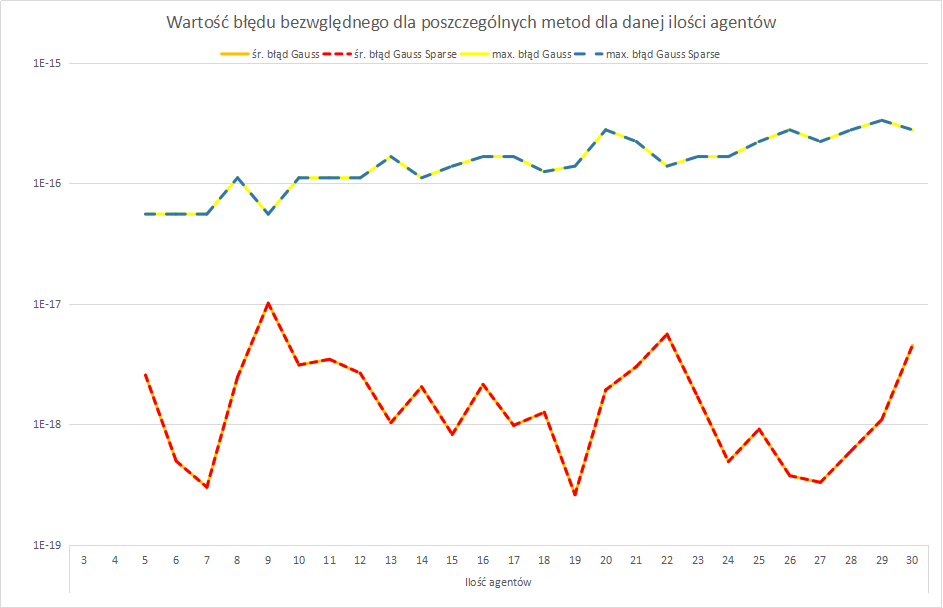
\includegraphics[width=\textwidth]{2.png}
		\caption{ \label{Rys2a}}
	\end{subfigure}
\end{figure}
\subsection{Analiza wyników}
Błąd bezwzględny dla poszczególnych metod był wyliczany w sposób następujący:
\begin{enumerate}
	\item Wygenerowana została macierz $A$ oraz wektor $B$
	\item Za pomocą danego
\end{enumerate}
\subsubsection{Gauss oraz Gauss z optymalizacją dla macierzy rzadkich}
\section{Podział pracy}
\centering
	\begin{tabular}{| p{4.4cm} | p{4.4cm} | p{4.4cm} |}
		\hline
		\textbf{Dawid Bińkuś} & \textbf{Oskar Bir} & \textbf{Mateusz Małecki} \\ \hline
		 \hline
		
		
		
	\end{tabular}
\end{document}